\documentclass[a4paper]{article}
\usepackage[utf8]{inputenc}
\usepackage[spanish]{babel} 
\renewcommand{\spanishtablename}{Tabla} 
\spanishdecimal{.}
\usepackage{verbatim}
\usepackage{amssymb}
\usepackage{subcaption}
\usepackage{wrapfig}
\usepackage{graphicx}
\usepackage{hyperref}
\usepackage{mathtools}
\usepackage{float}
\usepackage{siunitx}
\renewcommand{\thefootnote}{\arabic{fotnote}}
\setlength{\parskip}{\baselineskip} 
\usepackage{pdfpages}

\begin{document}

\begin{titlepage}
\paragraph{}

\begin{center}
\vspace*{0.10in}
\begin{figure}
\raggedleft

\includegraphics[scale=0.12]{unam.png}
\hspace{7.2cm}
\raggedright
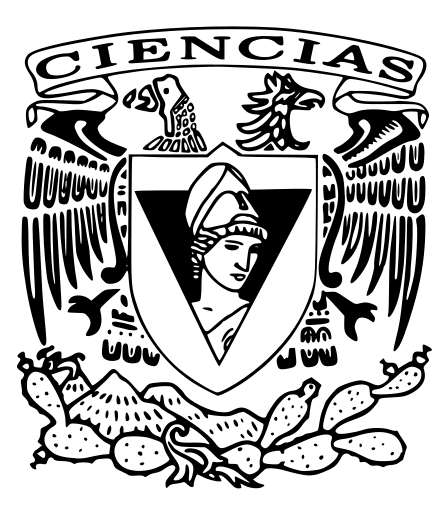
\includegraphics[scale=0.15]{fac.png}    
\end{figure}
\vspace*{0.5in}
UNIVERSIDAD NACIONAL AUTÓNOMA DE MÉXICO\\
\vspace*{0.2in}
FACULTAD DE CIENCIAS \\
\vspace*{0.5in}
\begin{large}
Laboratorio de Calor, Ondas y Fluidos\\
\end{large}
\vspace*{0.2in}
\begin{Large}
\textbf{Práctica 5} \\
\textbf{Calor de Vaporización.} \\
\end{Large}
\vspace*{0.3in}
\vspace*{0.3in}
\rule{80mm}{0.1mm}\\
\vspace*{0.1in}
\begin{large}
Profesor:  Quintanar Robles, Luis  \\
Ayudante: Quintanar Cortés, Luis Enrique \\
Mesa 1\\
Fecha de la práctica: 10 de septiembre de 2019.\\
Alumnos: León Arenal Sebastian.\\
Robledo Ibarra Emiliano. \\
Toledo Castañeda, Akim Tarik.\\

\end{large}
\end{center}
\end{titlepage}



\section*{Resumen.}
Se estudió la relación entre el calor suministrado por una resistencia eléctrica a un sistema termodinámico y la masa que varía con el tiempo del mismo . Se encontró una relación lineal entre el calor suministrado y la pérdida de masa del sistema, de tal manera que el calor suministrado $Q$ dividido entre la variación de la masa respecto al tiempo $\frac{\Delta m}{\Delta t}$ es constante. Se obtuvo un calor de vaporización de $(3900\pm100)\frac{J}{gr}$, sin embargo este dista demasiado del valor teórico $2260\frac{J}{gr}$. Por lo que se propone otro sistema con posibilidades de mediciones más precisas y con intercambio de materia con el exterior para observar el fenómeno a estudiar.


%%%%%%%%%%%%%%%%%%%%%%%%%%%%%%%%%%%%%%%%%%%%%%%%%%%%%%%%%%%%%%%%%%%%%%%%%%%%%%%%%%%%%%%%%%%%%%%%%%%%%%%%%%%%%%%%%%%%%%%%%%%%%%%%%%%%%%%%%%%%%%%%%%%%%%%%%%%%%%%%%%%%%%%%
\section*{Introducción.}
Un fenómeno usual en los materiales es cambiar de fase o estado de agregación, conforme agregamos calor a un material este puede dilatarse e inclusive deformarse.  Todos los materiales tienen una temperatura crítica que al llegar a esta el material comienza a cambiar de fase debido a la energía adquirida; la temperatura a la cual ocurre dicho fenómeno es distinta para cada material y esto se debe a sus características físicas y químicas. Es bien conocido que el agua se solidifica cuando su temperatura es menor o igual a cero grados Celsius y que comienza a evaporar cuando alcanza o rebasa los cien grados Celsius. Llamamos a este fenómeno calor latente y aplica tanto al cambio de estado sólido a líquido como de líquido a gas. Es necesario mencionar que cuando se habla de calor latente se está hablando que la energía en forma de calor se invierte para el cambio de fase y no para un aumento de la temperatura. Este documento se centrará en el cambio que ocurre de líquido a gas en el agua; a este fenómeno se le llama \textit{calor de vaporización} y se define como la energía necesaria para cambiar un gramo de sustancia en estado líquida, al estado gaseoso en el punto de ebullición. Este efecto del calor latente se debe a que esta energía suministrada rompe las fuerzas atractivas intermoleculares de manera que el estado de agregación del objeto cambia.

El objetivo primordial del presente es poder verificar si el calor suministrado es proporcional a la masa del objeto, esto es:
$$Q \propto m \quad \xrightarrow{} \quad Q=L_v m \quad \xrightarrow{} \quad L_v = \frac{Q}{m}$$
Donde $L_v$ es la constante a buscar tal que cumple con la ecuación. Se relacionará el trabajo (Joules) que se describe como la potencia (en este caso eléctrica) por unidad de tiempo, i.e. $W = Vi\Delta t$ y la pérdida continua de masa debido a la evaporación del agua.

%%%%%%%%%%%%%%%%%%%%%%%%%%%%%%%%%%%%%%%%%%%%%%%%%%%%%%%%%%%%%%%%%%%%%%%%%%%%%%%%%%%%%%%%%%%%%%%%%%%%%%%%%%%%%%%%%%%%%%%%%%%%%%%%%%%%%%%%%%%%%%%%%%%%%%%%%%%%%%%%%%%%%%%%
\section*{Procedimiento.}
Para poder realizar las mediciones se construyó un sistema de manera que este tuviera el menor intercambio de calor con el exterior, además, se buscó una forma de proveer calor al sistema de manera cuantificable y posible de regular, debido a ello se ocuparon dos instrumentos: un variac y un calorímetro. Para poder crear un sistema que fuera regulable se conectó un variac que controlaría toda fuente de energía suministrada al sistema. En el caso del control sobre la transferencia del calor se optó por mantener un calorímetro que guardara al sistema a medir de manera que los registros tomados fueron realizados a este instrumento, sobre todo en la medición continua del peso para poder obtener los cambios del mismo por cada lapso de tiempo, se estableció de un minuto.

Al variac se conectó una extensión construida de forma que la medición de voltaje y corriente mediante un multímetro (en modo de corriente alterna) fuera posible, luego se cerró el circuito con una resistencia y se comprobaron las mediciones; primero se decidió un voltaje e intensidad de la corriente para comprobar las conexiones y medidores: en la primera medición se decidió en $(19.8\pm0.05)V$ con $(5.06\pm0.005)A$ y para la segunda $(21.3\pm0.05)V$ con $(5.46\pm0.005)A$. Siempre se mantuvo la corriente menor a 6 amperes para no dañar ningún aparato y/o conexión.

\begin{figure}[H]
    \centering
    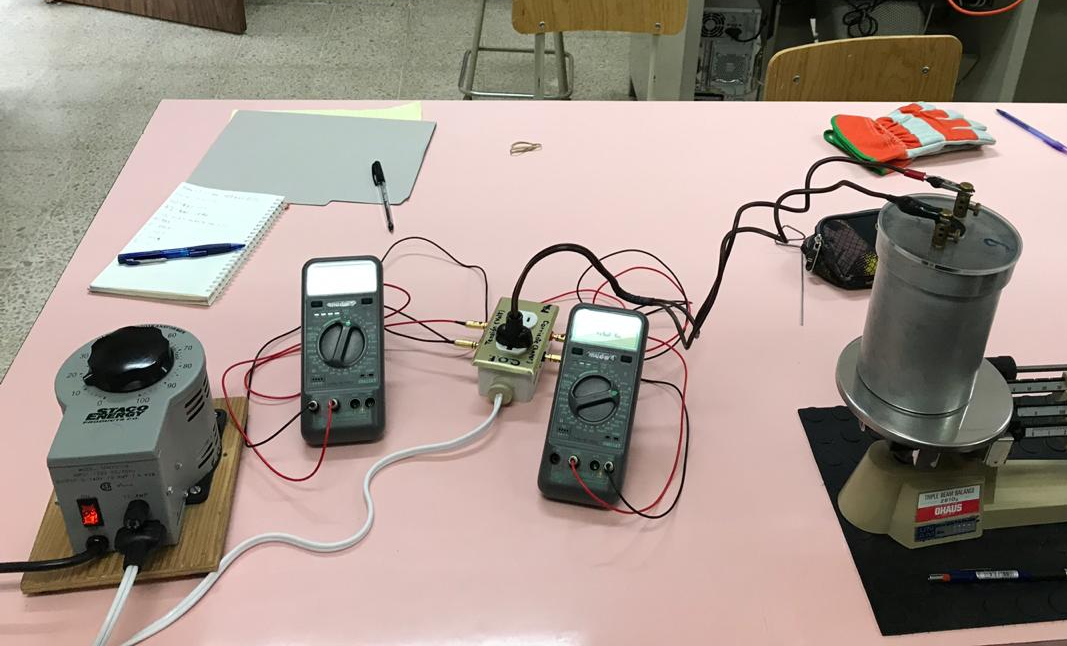
\includegraphics[width=11cm]{expe.png}
    \caption{Sistema aislado utilizado para las mediciones de temperaturas de equilibrio.}
\end{figure}

Se midió la masa del calorímetro, obteniendo una masa total de $(409.6\pm0.05)gr$, después se le colocó agua dentro para poder obtener el sistema de masa que variará, se midió su masa otra vez y luego se le colocaron las pinzas caimán a las resistencias para medir su masa una última vez. Se midió dos veces debido a que el peso que agregan los cables no es despreciable. Una vez regulada la energía y habiendo medido la masa del sistema se le comenzó a suministrar energía de forma constante, hasta observar pérdidas de masa en el mismo, una vez ocurrido esto se midió continuamente la masa y se registraron los datos de la masa del sistema cada minuto o tan próximo como se pudiera obtener.

En lo que refiere al análisis de datos se registraron desde que se activó la resistencia, para reconocer desde cuando la masa cambiaba, por razones de simplicidad sólo se consideraron tres medidas antes de que comenzara a cambiar la masa. Debido a que se midieron sistemas en conjunto y se requirió restar medidas las incertidumbres para cada masa quedan de la siguiente forma: la masa del calorímetro es $m_{cal} = (409.60\pm0.05)gr$, la masa del agua es $m_{agua} = (m_{cal + agua} - 409.6 \pm 0.1)gr$ y para la masa del sistema completo (con pinzas) $(m_{sis}\pm0.05)gr$. Para obtener la recta de ajuste se utiliizó Gnuplot y con ello la incertidumbre del mismo, por último, la constante de vaporización, debido a que fue obtenida de manera indirecta se utilizó la propagación de incertidumbres con la ecuación: $dL_v = \left|\frac{i}{a} \right|dV + \left|\frac{V}{a} \right|di +\left|\frac{Vi}{a^2} \right|da$. Donde $a$ es la pendiente del ajuste, $V$ el voltaje e $i$ la intensidad.

%%%%%%%%%%%%%%%%%%%%%%%%%%%%%%%%%%%%%%%%%%%%%%%%%%%%%%%%%%%%%%%%%%%%%%%%%%%%%%%%%%%%%%%%%%%%%%%%%%%%%%%%%%%%%%%%%%%%%%%%%%%%%%%%%%%%%%%%%%%%%%%%%%%%%%%%%%%%%%%%%%%%%%%%
\section*{Resultados.}
Aquí se muestran los datos extraídos de las dos mediciones realizadas la incertidumbre en el tiempo se muestra como $s_t = 1 s$ y la incertidumbre de la masa como $s_m = 0.05 gr$.
\subsubsection*{Primera medición.}
\begin{itemize}
    \item Voltaje utilizado: $V_i = (19.80\pm0.05)V$.
    \item Intensidad utilizada: $i = (5.060\pm0.005)A$.
    \item Masa inicial del sistema: $m = (747.30\pm0.05)gr$.
\end{itemize}
\begin{table}[H]
  \centering
    \begin{tabular}{|c|c|c|c|} \hline
    \multicolumn{1}{|l|}{Tiempo [s]} & \multicolumn{1}{|l|}{Masa [gr]} & \multicolumn{1}{|l|}{$s_t$ [s]} & \multicolumn{1}{|l|}{$s_m$ [gr]} \\ \hline
    0     & 747.30 & 1     & 0.05 \\ \hline
    60    & 747.30 & 1     & 0.05 \\ \hline
    120   & 747.30 & 1     & 0.05 \\ \hline
    180   & 747.00 & 1     & 0.05 \\ \hline
    240   & 746.10 & 1     & 0.05 \\ \hline
    300   & 744.70 & 1     & 0.05 \\ \hline
    360   & 743.60 & 1     & 0.05 \\ \hline
    420   & 742.00 & 1     & 0.05 \\ \hline
    480   & 740.30 & 1     & 0.05 \\ \hline
    540   & 739.00 & 1     & 0.05 \\ \hline
    627   & 738.20 & 1     & 0.05 \\ \hline
    660   & 737.30 & 1     & 0.05 \\ \hline
    730   & 736.00 & 1     & 0.05 \\ \hline
    780   & 734.50 & 1     & 0.05 \\ \hline
    840   & 733.00 & 1     & 0.05 \\ \hline
    900   & 732.30 & 1     & 0.05 \\ \hline
    960   & 731.00 & 1     & 0.05 \\ \hline
    1020  & 729.20 & 1     & 0.05 \\ \hline
    1080  & 727.10 & 1     & 0.05 \\ \hline
    1140  & 725.60 & 1     & 0.05 \\ \hline
    1200  & 723.20 & 1     & 0.05 \\ \hline
    1260  & 721.80 & 1     & 0.05 \\ \hline
    1320  & 719.20 & 1     & 0.05 \\ \hline
    \end{tabular}%
  \caption{Mediciones del cambio de la masa respecto al tiempo del primer sistema.}
\end{table}%

\begin{figure}[H]
    \centering
    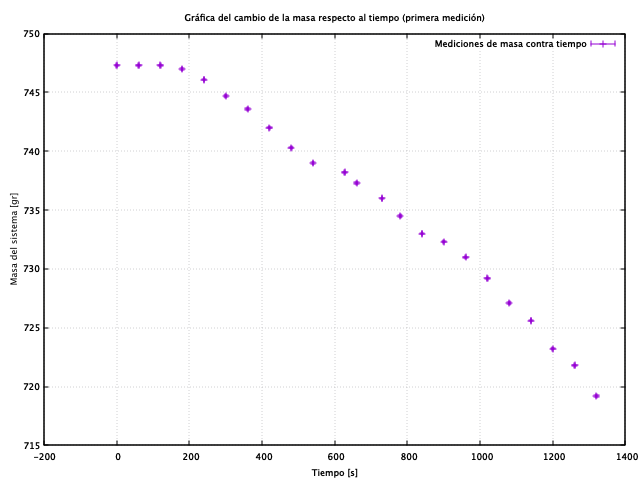
\includegraphics[width=11cm]{primeramed.png}
    \caption{Mediciones sistema aislado utilizado para las mediciones de temperaturas de equilibrio (primero sistema).}
\end{figure}
Se le hizo un ajuste a los puntos obtenidos de la primera medición y se obtuvo una recta con pendiente negativa. $m=-0.0234\pm0.0006$ y con ordenada al origen $b=752.1\pm0.5$.\\
Con los datos obtenidos en la primera medición, se obtuvo un calor de vaporización ${{L}_v}_1=(4200\pm100)\frac{J}{gr}$
\begin{figure}[H]
    \centering
    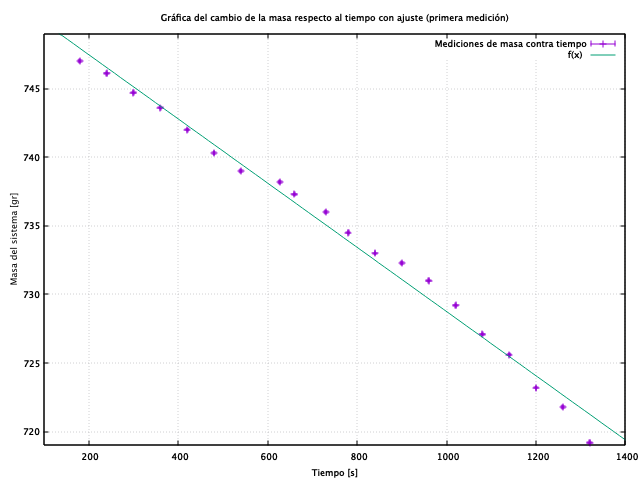
\includegraphics[width=11cm]{primeraajuste.png}
    \caption{Recta ajustada de la primera medición.}
\end{figure}
%%%%%%%%%%%%%%%%%%%%%%%%

\subsubsection*{Segunda medición.}
\begin{itemize}
    \item Voltaje utilizado: $V_i = (21.30\pm0.05)V$.
    \item Intensidad utilizada: $i = (5.460\pm0.005)A$.
    \item Masa inicial del sistema: $m = (827.40\pm0.05)gr$.
\end{itemize}
\begin{table}[H]
  \centering
    \begin{tabular}{|c|c|c|c|} \hline
    \multicolumn{1}{|l|}{Tiempo [s]} & \multicolumn{1}{|l|}{Masa [gr]} & \multicolumn{1}{|l|}{$s_t$ [s]} & \multicolumn{1}{|l|}{$s_m$ [gr]} \\ \hline
    0     & 827.40 & 1     & 0.05 \\ \hline
    60    & 827.40 & 1     & 0.05 \\ \hline
    120   & 827.40 & 1     & 0.05 \\ \hline
    180   & 827.30 & 1     & 0.05 \\ \hline
    240   & 825.20 & 1     & 0.05 \\ \hline
    300   & 824.20 & 1     & 0.05 \\ \hline
    360   & 822.50 & 1     & 0.05 \\ \hline
    420   & 820.30 & 1     & 0.05 \\ \hline
    480   & 818.60 & 1     & 0.05 \\ \hline
    540   & 816.90 & 1     & 0.05 \\ \hline
    600   & 814.90 & 1     & 0.05 \\ \hline
    660   & 813.00 & 1     & 0.05 \\ \hline
    720   & 811.10 & 1     & 0.05 \\ \hline
    780   & 809.40 & 1     & 0.05 \\ \hline
    870   & 806.50 & 1     & 0.05 \\ \hline
    900   & 805.50 & 1     & 0.05 \\ \hline
    960   & 803.20 & 1     & 0.05 \\ \hline
    1020  & 801.30 & 1     & 0.05 \\ \hline
    \end{tabular}%
  \caption{Mediciones del cambio de la masa respecto al tiempo del segundo sistema.}
\end{table}%

\begin{figure}[H]
    \centering
    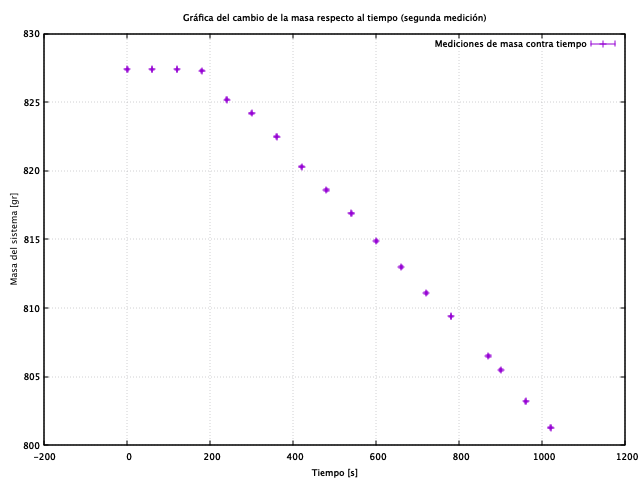
\includegraphics[width=11cm]{segundamed.png}
    \caption{Mediciones del sistema aislado utilizado para las mediciones de temperaturas de equilibrio (segundo sistema).}
\end{figure}

Se hizo un ajuste con los datos obtenidos en la segunda medición y se obtuvo una recta con pendiente negativa $m=-0.0309\pm0.0003$ y ordenada al origen $b=833.3\pm0.2$\\
Con los datos obtenidos en la segunda medición, se obtuvo un calor de vaporización ${{L}_v}_2=(3760\pm50)\frac{J}{gr}$
\begin{figure}[H]
    \centering
    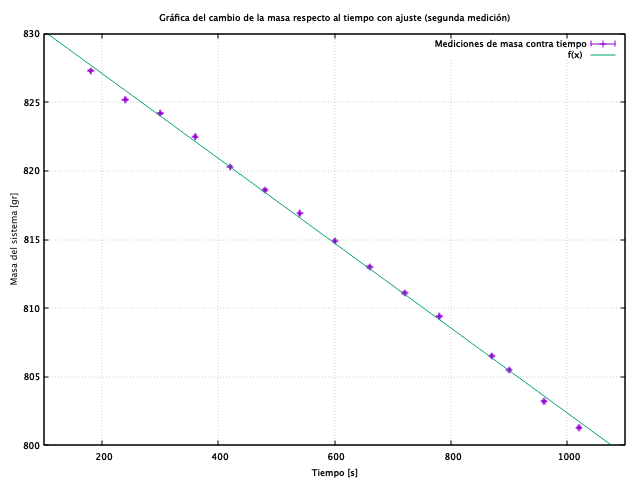
\includegraphics[width=11cm]{segundaajuste.png}
    \caption{Recta ajustada de la segunda medición.}
\end{figure}
Al obtener los calores de vaporización ${{L}_v}_1$ y ${{L}_v}_2$, se calculará el calor de vaporización promedio ${{L}_v}_p=(3900\pm100)\frac{J}{gr}$, que se utilizará como valor de comparación. 

%%%%%%%%%%%%%%%%%%%%%%%%%%%%%%%%%%%%%%%%%%%%%%%%%%%%%%%%%%%%%%%%%%%%%%%%%%%%%%%%%%%%%%%%%%%%%%%%%%%%%%%%%%%%%%%%%%%%%%%%%%%%%%%%%%%%%%%%%%%%%%%%%%%%%%%%%%%%%%%%%%%%%%%%
\section*{Conclusiones.}
Al obtener el calor de vaporización promedio se puede observar que el coeficiente obtenido dista demasiado del valor teórico (valor teórico $2260 J/gr$) lo cual nos lleva a pensar en dos alternativas: la primera y con mayor peso es que el sistema usado no es el más idóneo, la segunda opción es cuestionar la teoría. Debido a que es más probable que se haya cometido un error en el sistema en el apartado de la masa, debido a que se midió la masa del calorímetro, este necesitaba estar cerrado por lo cual las aberturas que el sistema tenía fueron lo suficientemente pequeñas como para que aunque escapara la masa de forma constante, limitara este fenómeno de pérdida de masa por lo cual en realidad la medición que se obtuvo fue completamente sesgada debido al recipiente aislante.

Debido a que ambas mediciones fueron realizadas con el mismo sistema las dos mediciones obtenidas son cercanas entre sí pero no son congruentes con el valor esperado (teórico), es por ello que para mejorar el experimento se propone utilizar un recipiente no aislante, con una abertura para poder dejar libre al exterior y ver este cambio de masa más pronunciado. Otro aspecto importante en la medición fue el continuo problema de la masa, se utilizó una balanza granataria, sin embargo, debido a que es un instrumento de calibración manual, ocurrían dos fenómenos relevantes durante la cuantificación con la misma: la primera es la más conocida y es que debido a que requiere ser ajustada continuamente y se debe esperar a que se estabilice esto genera cierta incertidumbre con respecto al valor obtenido y la segunda es sobre el instrumento mismo, es bien sabido que con cada medición se va descalibrando el instrumento por lo que al final de las mediciones era posible constatar que el valor en el que debería marcar cero gramos no era correcto. Esto cobra significado ya que muestra errores claros que invalidan los resultados. Finalmente se propone repetir el experimento cambiando el sistema en la parte de la medición de la masa con instrumentos de mayor confianza, esto es, una balanza electrónica que pueda soportar el calor y el envase contenedor de la sustancia a observar que podría ser sustituido con un matraz por ejemplo.

El resultado obtenido, bajo la interpretación que toma en cuenta lo dicho anteriormente, es en realidad como varía la masa dentro del recipiente con un material (en este caso agua) que puede evaporarse, esta relación entre disminución de materia y tiempo es constante para todo tiempo en ambas mediciones, esto lleva a un resultado en el que podemos asegurar que el cambio de la masa respecto al tiempo se encuentra directamente relacionado con la energía aplicada al sistema, esto podemos verlo en los ajustes realizado y la pendiente obtenida. De manera que proponemos esta conclusión ya que no fue fructífero el experimento con el resultado esperado.
%%%%%%%%%%%%%%%%%%%%%%%%%%%%%%%%%%%%%%%%%%%%%%%%%%%%%%%%%%%%%%%%%%%%%%%%%%%%%%%%%%%%%%%%%%%%%%%%%%%%%%%%%%%%%%%%%%%%%%%%%%%%%%%%%%%%%%%%%%%%%%%%%%%%%%%%%%%%%%%%%%%%%%%%
\section*{Bibliografía}
Oda, B.,  Universidad Nacional Autónoma de México. Facultad de Ciencias. (2005). Introducción al análisis gráfico de datos experimentales (3ª ed.). Ciudad de México, México: UNAM, Facultad de Ciencias.

Resnick, R., Halliday, D., Krane, K. (2001). \textit{Física Vol. 1}. ($4^a$ ed). México. GRUPO PATRIA CULTURAL
\end{document}


